\chapter{Unendlichdimensionale Vektorräume}
\label{sec:unendliche VRs}
Dieses Kapitel stellt die Schnittstelle zwischen linearer Algebra und Funktionalanalysis dar, welche sich mit unendlichdimensionalen \aclp{VR} beschäftigt. 
\section{Funktionenvektorraum}

\begin{Satz} vgl.\,\cite[S. 28 f., 6.2]{Skript} (\emph{Der reelle Funktionenraum}) \label{funktionenraum}Die Menge aller reellen Funktion\footnote{In der Schule behandeln wir ausschließlich reelle Funktionen mit der Defintions- und Wertemenge $\mathbb{R}$.}
\[F \vcentcolon=  \Abb(\mathbb{R}, \mathbb{R})\vcentcolon= \{f : \mathbb{R} \rightarrow\mathbb{R}\}\]
bilden einen \acl{VR} über den Körper der reellen Zahlen $\mathbb{R}$ mit folgender Definition von Addition und Skalarmultiplikation:
\begin{enumerate}
	\item Die Addition $f+g\in F$ für $f,g \in F$ definieren wie als
	\begin{align*} (f+g)(x) \vcentcolon= f(x)+ g(x)\text{.}
	\end{align*}
	
	\item Die Skalarmultiplikation $\lambda \cdot f \in F$ für $\lambda \in \mathbb{R}$ und $f \in F$ definieren wir als 
	
	\[(\lambda \cdot f)(x) \vcentcolon= \lambda \cdot f (x)\text{.}\]		
\end{enumerate}
\end{Satz}

Anstatt Vektoren als Verschiebungvorschriften von Punkten wie in $\mathbb{R}^2$ oder $\mathbb{R}^2$ hat der Funktionenraum einzelne Funktionen als "Vektoren", die sich genauso addieren und skalamultiplizieren lassen.
\newpage
\begin{example}
Wird eine Funktion mit einer Konstanten addiert, wird sie in $y$-Richtung nach oben (wie in Abbildung \ref{fig:fadd}) oder nach unten verschoben.
\end{example}
\begin{figure}[h]
\begin{minipage}[h]{.5\textwidth}
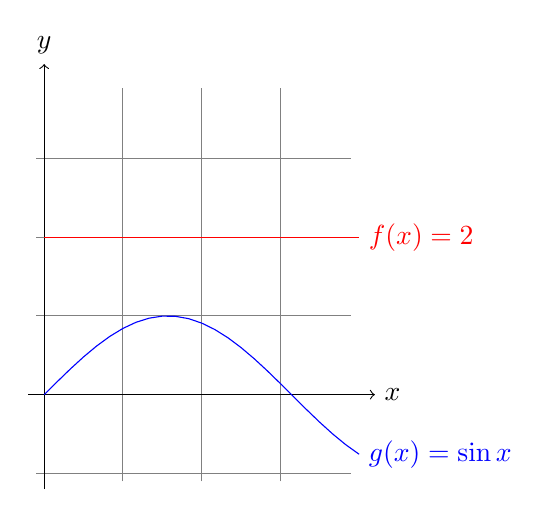
\begin{tikzpicture}[domain=0:4] 
	\draw[color=gray] (-0.1,-1.1) grid (3.9,3.9);
	\draw[->] (-0.2,0) -- (4.2,0) node[right] {$x$}; 
	\draw[->] (0,-1.2) -- (0,4.2) node[above] {$y$};
	\draw[color=red] plot (\x,2) node[right] {$f(x) =2$}; % \x r means to convert ’\x’ from degrees to _r_adians: 
	\draw[color=blue] plot (\x,{sin(\x r)}) node[right] {$g(x) = \sin x$}; 
\end{tikzpicture}
\end{minipage}
\hfil
\begin{minipage}[h]{.5\textwidth}
\begin{tikzpicture}[domain=0:4] 
	\draw[color=gray] (-0.1,-1.1) grid (3.9,3.9);
	\draw[->] (-0.2,0) -- (4.2,0) node[right] {$x$}; 
	\draw[->] (0,-1.2) -- (0,4.2) node[above] {$y$};
	 % \x r means to convert ’\x’ from degrees to _r_adians: 
	\draw[color=violet] plot (\x,{sin(\x r)+2}) node[right] {$(f+g)(x) = 2+\sin x$}; 
\end{tikzpicture}
\end{minipage}
\caption{Funktionenaddition}
\label{fig:fadd}
\end{figure}

\begin{example}
Im Falle von Abbildung \ref{fig:fskl} wird die Sinus-Funktion in $y$-Richtung gestreckt, indem ihre Amplitude durch die Skalarmultiplikation verdoppelt wird.
\end{example}
\begin{figure}[h]
\centering
\begin{tikzpicture}[domain=0:4] 
	\draw[color=gray] (-0.1,-1.1) grid (3.9,3.9);
	\draw[->] (-0.2,0) -- (4.2,0) node[right] {$x$}; 
	\draw[->] (0,-1.2) -- (0,4.2) node[above] {$y$};
	\draw[color=blue] plot (\x,{2*sin(\x r)}) node[right] {$2 \cdot g(x) =2 \cdot \sin x$}; 
\end{tikzpicture}
\caption{Funktionenskalarmultiplikation}
\label{fig:fskl}
\end{figure}

\newpage
\begin{proof}
Vor.: Funktionenaddition und Funktionenskalarmultiplikation von \ref{funktionenraum} werden für alle Beweise benötigt.
\\ Beh.: $F$ ist ein $\mathbb{R}$-\acl{VR}.
\\ Bew.: Wir müssen $F$ auf alle Vektorraumaxiome (siehe \ref{VR-axiome}) hin überprüfen. Aus der Definition von $F$ folgt: \(f(x) \in \mathbb{R}\) für alle $f$. Die Ergebnisse aller Funktionen aus $F$ sind reelle Zahlen, somit haben sie alle Körpereigenschaften (siehe \ref{Koerper}). Wir können mit ihnen wie gewohnt rechnen. Zuerst zeigen wir, dass $(F,+)$ eine abelsche Gruppe (vgl. \ref{Gruppe}, \ref{abl.Gruppe}) ist.
\\Für alle $f,g,h \in F$ und $\lambda_1, \lambda_2 \in \mathbb{R}$ gilt:
\begin{enumerate}
\item (Assoziativität)
\( ((f+g)+h)(x)=(f+g)(x)+h(x)=f(x)+g(x)+h(x)=\\f(x)+(g(x)+h(x))=(f+(g+h))(x)\)
\item(Existenz des neutralen Elements) Sei $0_{\Abb}(x)=0$ für alle $x \in \mathbb{R}$.\footnote{Wir bezeichnen diese Funktion als die sogenannte "Nullabbildung", die alle Elemente auf $0$ abbildet. Ihr Graph ist die $x$-Achse.} \\ \( (0_{\Abb}+f)(x) = 0_{\Abb}(x) + f(x)= 0+ f(x)=f(x)=f(x)+0=f(x)+ 0_{\Abb}(x)=(f+0_{\Abb})(x) \)
\item(Existenz des Inversen) Sei $-f \in F$ das Inverse für alle $f\in F$.\footnote{Wird eine beliebige Funktion an der $x$-Achse gespiegelt, also mit $-1$ skalarmultipliziert, entsteht das Inverse.}
\\ \( (f+(-f))(x) =  f(x) + (-f(x))= f(x)-f(x) = 0_{\Abb}(x) =  (-f(x)) + f(x)= ((-f) + f)(x)\) 
\item(Kommutativität) \((f+g)(x)=f(x)+g(x)=g(x)+f(x)=(g+f)(x)\)
\end{enumerate}

Es müssen noch die Eigenschaften eines \acl{VR}es gezeigt werden.
\begin{enumerate}
\item \((\lambda_1+\lambda_2)\cdot f(x) = \lambda_1 \cdot f(x) + \lambda_2 \cdot  f(x)\)
\item \( \lambda_1 \cdot (f + g)(x) = (\lambda_1 \cdot f + \lambda_1 \cdot  g)(x) = \lambda_1 \cdot f(x) + \lambda_1 \cdot  g(x)\)
\item \( \lambda_1 \cdot (\lambda_2 \cdot f(x)) = (\lambda_1 \cdot \lambda_2) \cdot f(x) \)
\item \(1 \cdot f(x) = f(x)\)
\qedhere
\end{enumerate}
\end{proof}
%%%%%%%%%%%%%%%%%%%%%%%%%%%%%%%%%%%%%%%%%%%%%%%%%%%%%%%%%%%%%%%%%%%%%%%%%%%%%%%%%%%%%%%%%%%%%%%%%%%%%%%%%%%%%%%%%%%%%%%%%%%%%%
\newpage
\section{Polynomvektorraum}
\label{sec:RX}
Um eine intuitive Vorstellung von dem Funktionenraum aller reellen Funktionen zu erlangen, beschäftigen wir uns zunächst mit einer Teilmenge von $F$, den Polynomen $\acl{RX}$, die ebenso Abbildungen von $\mathbb{R}\rightarrow \mathbb{R}$ sind.
\theoremstyle{definition}
\begin{definition}vgl.\,\cite[S. 44, 1.28]{Springer} (\emph{Polynome}) \label{def:Polynome}Ein Polynom vom Grad $\leq n$ hat die Form \[f(x)= \sum\limits_{i=0}^{n} \lambda_i x^i = \lambda_0 + \lambda_1 x + \lambda_2 x^2 + ... + \lambda_n x^n \] für $\lambda_i \in \mathbb{R}$.
\end{definition}

\begin{Satz}vgl.\,\cite[S. 44f., 1.28]{Springer} (\emph{Polynomvektorraum $\mathbb{R}[x]$}) \label{PVR}Die Menge aller Polynome aus \ref{def:Polynome} bezeichnen wir als $\mathbb{R}[x]$. Sie bildet einen $\mathbb{R}$-\acl{UVR} (siehe \ref{UVR}) mit der Definition von Addition und Multiplikation aus \ref{funktionenraum}:
\begin{enumerate}

\item (Polynomaddition) Für alle \(f(x)=\sum\limits_{i=0}^{n} \mu_i x^i\text{,}\; g(x)=\sum \limits_{i=0}^n \nu_i x^i\) gilt:
\begin{align*}(f+g)(x) = \sum_{i=0}^{n}\mu_i x^i + \sum_{i=0}^{n} \nu_i x^i = \sum_{i=0}^{n} (\mu_i + \nu_i)x^i \text{.}\end{align*}
\item (Polynomskalarmultiplikation)
Seien $f(x) \in \acl{RX}$ beliebig und $\lambda \in \mathbb{R}$.
\begin{align*}
(\lambda \cdot f) (x) = \lambda \cdot \sum_{i=0}^{n} \mu_i x^i= \sum_{i=0}^{n} \lambda \cdot \mu_i x^i\text{.}
\end{align*}
\end{enumerate}
\end{Satz}

\begin{proof}
Vor.: Pplynomaddition und -skalarmultiplikation aus \ref{PVR}.
\\ Beh.: siehe Satz \ref{PVR}
\\ Bew.: Wir rechnen die Axiome aus \ref{UVR} für $\acl{RX}$ durch.
\\ Seien $u(x)=\sum\limits_{i=0}^{n} \zeta_i x^i\text{,}\; v(x) = \sum\limits_{i=0}^{n} \eta_i x^i \in \acl{RX}$ beliebig.
\begin{enumerate}
\item Zu zeigen gilt, dass der Nullvektor ein Element von $\acl{RX}$ ist. Sei $\rho = 0$. \[\rho \cdot u(x)= 0 \cdot \sum\limits_{i=0}^{n} \zeta_i x^i = 0_{\Abb}(x) \Rightarrow 0_{\Abb}(x) \in \acl{RX}\]
\item Es gilt die Abgeschlossenheit der Polynomaddition zu beweisen.
\\ \[ (u+v)(x)=u(x) + v(x) = \sum\limits_{i=0}^{n} \zeta_i x^i+\sum\limits_{i=0}^{n} \eta_i x^i =\sum\limits_{i=0}^{n} (\zeta_i+ \eta_i )x^i \in \acl{RX} \]
\item Die Skalarmultiplikation soll auf ihre Abgeschlossenheit hin getestet werden. Sei $\varrho \in \mathbb{R}$ beliebig.
\[(\varrho \cdot u)(x) = \varrho \cdot u(x)= \varrho \cdot \sum\limits_{i=0}^{n} \zeta_i x^i\ = \sum\limits_{i=0}^{n} \varrho \cdot \zeta_i x^i \in \acl{RX}\qedhere\]
\end{enumerate}
\end{proof}
Wir benötigen eine Basis, um die Dimension des \acl{PV}es zu bestimmen. 
\theoremstyle{Lemma}
\begin{Lemma}({\emph{Basis von $\acl{RX}$}}) Die Menge aller Monome $1, x, x^2,…, x^n$ vom Grad $\leq n$ bildet eine Basis $B_{\acl{RX}}$ des \acl{PV}es. 
\end{Lemma}
%\newpage
\begin{proof}
\label{BewBas}
Vor.: Theo. \ref{theo:Basis} (\ref{Basis1}), Def. \ref{def:Polynome}, Def. \ref{def:linunab}
\\ Beh.: Die Menge $B_{\acl{RX}}\vcentcolon=\{1, x, x^2,…, x^n\}$ sei eine Basis des Polynomvektorraums.
\\ Bew. vgl. \cite[S. 308]{Tut}.: Wir müssen überprüfen, ob die Menge \acl{linunab} und ein \acl{EZS} ist.  
\\ \acl{Linunab}:
\\ Es ist zu zeigen, dass die Gleichung \begin{equation}\label{GLS} \sum\limits_{i=0}^n \lambda_i x^i = \lambda_0 + \lambda_1 x + ... + \lambda_n x^n = 0\end{equation} nur für alle $\lambda_i=0$ mit $i \in \mathbb{N}_0$ lösbar ist.\footnote{Wir müssen ein Gleichungssystestem mit $n$ Variablen schrittweise lösen.}
\begin{enumerate}
\item \label{S1} Setze zunächst $x=0$ in (\ref{GLS}). 
\begin{equation}\Rightarrow \lambda_0 + \lambda_1 \cdot 0 + \lambda_2 \cdot 0^2 + ... + \lambda_n \cdot 0^n\ \Rightarrow \lambda_0 = 0 \end{equation}
\item \label{GLS2} Setze $\lambda_0$ in (\ref{GLS}) ein. 
\begin{align}
\Rightarrow\lambda_1 \cdot x + \lambda_2 \cdot x^2+ ... + \lambda_n \cdot x^{n-1} = 0 
\end{align} Wir dürfen (\ref{GLS2}) nun durch $x$ teilen, wenn $x\not= 0$ ist: 
\begin{align}
\lambda_1 \cdot x + \lambda_2 \cdot x^2 +... + \lambda_n  \cdot x^n &= 0 && |:x \\ \Rightarrow \lambda_1 + \lambda_2 \cdot x+ ... + \lambda_n \cdot x^{n-1} &= 0
\end{align}
\end{enumerate}
Wiederhole (\ref{S1}) und (\ref{GLS2}), solange bis alle $\lambda_i=0$ mit $i \in \mathbb{N}_0$ sind.
Somit ist die lineare Unabhängigkeit von $B_{\acl{RX}}$ gezeigt. \qed
\\ \acl{EZS}: Aus Def. \ref{def:Polynome} ist ersichtlich, dass jede Polynomfunktion $f(x)$ eine Linearkombination der Monome $1, x,x^2 …, x^n$ vom Grad $\leq n$ ist. Folglich bildet $B_{\acl{RX}}$ ein \acl{EZS}.
\end{proof}

\newpage
\section{Unendliches \acl{EZS}}
\theoremstyle{prop}
\begin{prop} \label{propunendl} Das \acl{EZS} von $\acl{RX}$ bestehend aus der Teilmenge $B_{\acl{RX}}=\{1, x,x^2 …, x^n\}\subset\acl{RX}$ ist unendlich.
\end{prop}


\begin{proof} 
Wir wollen mit einem Widerspruchsbeweis zeigen, dass das System $B_{\acl{RX}}$ unendlich erzeugt ist.
\\Vor.: Im vorigen Beweis wurde bereits überprüft, dass $B_{\acl{RX}}$ ein \textbf{\acl{EZS}} ist. 
\\Beh.: siehe Prop. \ref{propunendl}
\\Bew. vgl.  \cite[S.498 f.]{Enzy}: Angenommen, $B_{\acl{RX}}$ sei ein endliches \acl{EZS}. Somit gibt es ein Polynom vom maximalen Grad $n$. Das "nächsthöhergradige" Polynom vom Grad $n+1$ lässt sich allerdings nicht mehr durch eine \acl{Linkomb} von $B_{\acl{RX}}$ darstellen. Dies ist ein Widerspruch dazu, dass $B_{\acl{RX}}$ ein \textbf{\acl{EZS}} ist.\footnote{Die Basis $B_{\acl{RX}}$ müsste alle Polynome "linear kombinieren" können.} So folgt die Behauptung.
\end{proof}

\theoremstyle{Corollar}
\begin{Corollar}{ }
Aus der Definition des Dimensionenbegriffs in \ref{def:dim} schließen wir aufgrund des unendlichen \acl{EZS}s von $B_{\acl{RX}}$, dass $\dim(\acl{RX})= \infty$ ist. 
\end{Corollar}

%%%%%%%%%%%%%%%%%%%%%%%%%%%%%%%%%%%%%%%%%%%%%%%%%%%%%%%%%%%%%%%%%%%%%%
\section{Abzählbar unendliche Dimension}

\theoremstyle{prop}
\begin{prop}{ }
Die Dimension des reellen Polynomvektorraumes $\acl{RX}$ lautet: \begin{align*}\dim(\acl{RX})=\aleph_0\text{.} \end{align*}
\end{prop}

\begin{proof}
Vor.: Aus dem W-Seminarunterricht wissen wir, dass eine Menge $M$ genau dann abzählbar ist, wenn $|M|=|\mathbb{N}_0|=\aleph_0$ gilt.
\\Beh.: Die Basis $B_{\acl{RX}}$ ist abzählbar.
\\Bew.: Wir konstruieren eine eineindeutige\footnote{Zur Erinnerung: Jedem Element wird genau ein Element aus der Wertemenge zugeordnet. Wir sagen stattdessen auch "bijektiv".} Funktion:
\begin{align*}
\alpha: B_{\acl{RX}} &\rightarrow \mathbb{N}_0
\\ x^n &\mapsto n \end{align*}
\(\Rightarrow |B_{\acl{RX}} |=\aleph_0 \Rightarrow \dim(\acl{RX})=\aleph_0\) 
\end{proof}
\newpage
\section{Überabzählbar unendliche Dimension}
Wir wollen im Folgenden berechnen, welche Dimension $F$ hat. Da wir wissen, dass $\acl{RX}$ ein \acl{UVR} von $F$ ist, muss $\dim(F)\geq\dim(\acl{RX})$ sein. Hierfür bezeichnen wir die Mächtigkeit der reellen Zahlen als $|\mathbb{R}|=\vcentcolon\mathfrak{c}$.

\begin{Lemma} \label{fm} Seien $A$ und $B$ beliebige Mengen. Die Gesamtanzahl $G_F$ der Funktionen von $A \rightarrow B$ ist 
\begin{align*}
G_F= |A|^{|B|}.
\end{align*}
\end{Lemma} 

\begin{proof}
Aus den Axiomen der Kombinatorik kann man die Behauptung ableiten.
Seien $M=\{a,b,c\}$ und {$N=\{d,e,f,g\}$} Mengen. Wir wollen die Anzahl der Abbildungen von $M \rightarrow N$ ausrechnen.\footnote{Man kann sich die Abbildung der einzelnen Elemente aus der Definitons- zur Wertemenge beliebig definieren. Dabei muss man beachten, dass jedes Element einem anderen zugeordnet wird und nicht gleichzeitig auf mehr als zwei abgebildet wird.} Das Element $a$ hat vier Möglichkeiten, abgebildet zu werden, nämlich auf $d,e,f$ oder $g$. Analog gilt es für $b$ und $c$. So gibt es insgesamt $3^4=81$ Möglichkeiten, wie $a,b,c$ abgebildet werden können.\footnote{Der Beweis ist nicht allgemein. Er würde vertiefte Kenntnisse in die Kardinalarithmetik (Rechenregeln mit Kardinalzahlen) voraussetzen. Hier betrachten wir nur einen Spezialfall, der den Sachverhalt veranschaulichen soll.}
\end{proof}

\begin{Satz}vgl.\,\cite[S. 3, 3.2 (a)]{Card}\label{dim}
Sei $V$ ein $K$-\acl{VR}. Ist $|V|>|K|$, dann ist $|V|=\dim(V)$.
\end{Satz}

\begin{Corollar}
Die Mächtigkeit des Vektorraums $|F|$ ist die Anzahl aller reellen Funktionen von $\mathbb{R}\rightarrow\mathbb{R}$ (siehe Satz \ref{fm}). Dies entspricht:
\begin{align*}
|\mathbb{R}|^{|\mathbb{R}|}= \mathfrak {c}^{\mathfrak {c}} \text{.}  
\end{align*} 
Der Körper von $F$ ist $\mathbb{R}$. Somit gilt: 
\begin{align*}\mathfrak {c}^{\mathfrak {c}} > \mathfrak {c} \Rightarrow |F|>|\mathbb{R}|  \Rightarrow |F|=\dim(F)=\mathfrak {c}^{\mathfrak {c}}\text{.} \end{align*}
\end{Corollar}



%c {\displaystyle {\mathfrak {c}}} 











